\chapter{Unranking Restricted Permutations}
\label{cha:UnrankingMenage}
TODO

\section{TODO}
\begin{enumerate}
  \item Introduction
  \item Define \textbf{derived} complementary board $B_\alpha^c$?
  \item If we do a cyclic rotation of the rows of a chessboard, we get
    essentially the same thing.
  \item Move code to Appendix.
  \item Define $B_\alpha$ and $\overline{B}_\alpha^c$.
  \item Do we want to talk about parking functions?
  \item Is it worthwhile to discuss prefix functions for compositions, etc.?
  \item Make sure ``derank'' doesn't occur anywhere.
  \item Gives a way of sampling uniformly at random.
\end{enumerate}

% %%%%%%%%%%%%%%%%%%%%%%%%%%%%%%%%%%%%%%%%%%%%%
% Section 1
% %%%%%%%%%%%%%%%%%%%%%%%%%%%%%%%%%%%%%%%%%%%%%
\section{Overview and History}

In January 2020, Richard Arratia sent out an email announcing a talk he was
going to give on de-ranking derangements.

By January 2021, he announced a \$100 prize for solving the analogous problem
with m\'enage permutations. I solved that too.

Richard was interested in a more general question, which I found contagious:
Given some family of combinatorial objects that can be quickly counted
(say unlabelled simple graphs on $n$ vertices)
and some total ordering on them,
when is it possible to \textbf{unrank} the collection in some computationally
efficient way?

\begin{definition}
  Let $\mathcal C$ be a totally ordered finite set, and
  let $\{c_i\}_{i=1}^{|\mathcal C|}$ be the unique sequence of elements in
  $\mathcal{C}$ such that $c_i < c_{i+1}$ for all $1 \leq i < |\mathcal{C}|$.

  The \textbf{ranking map} is the map
  $\operatorname{rank}_{\mathcal{C}} \colon \mathcal{C} \rightarrow \mathbb N_{>0}$
  which sends $c_i \mapsto i$.

  The \textbf{unranking map} is the inverse map
  $\operatorname{unrank}_{\mathcal{C}} \colon \mathbb N_{>0} \rightarrow \mathcal{C}$
  which sends $i \mapsto c_i$.
\end{definition}

In abstract terms, these maps are not particularly interesting, but in practical
terms it can be quite difficult to efficiently compute a given ranking or
unranking from a given totally ordered set. After all, when these sets
grow in exponential time or worse, explicitly constructing the sequence and
doing a search is not computationally feasible.

In Appendix TODO, we will provide examples of total orders on combinatorial
objects $\mathcal{C}$ for which constructing efficient

% Of course, we can usually create an algorithm to give the $i$-th object without
% simply enumerating all of the objects explicitly? We want to ``jump in'' to a
% specific place on the list. Another interesting question:
% what if you get to supply both the total order and the unranking algorithm?

In this chapter we're going to explore that idea. We're going to show a general
theory that allows us to de-rank
permutations in lexicographic order,
derangements in lexicographic order,
partitions and compositions of $n$ in lexicographic order,
labeled trees by lexicographic order of Pr\"ufer code,
Lyndon words \cite{Kociumaka2014} (de Bruijn Sequences?),
Dyck path in lexicographic order?
% %%%%%%%%%%%%%%%%%%%%%%%%%%%%%%%%%%%%%%%%%%%%%
% Section 2
% %%%%%%%%%%%%%%%%%%%%%%%%%%%%%%%%%%%%%%%%%%%%%
\section{Prefix Counting and Word Ranking}

% If we can efficiently count how many objects in
% $[n]^k$ start with a given prefix
% (in $O(T(n,k))$ time),
% then we can just walk down the possible letters until
% we get to the right spot ($O(nkT(n,k))$).

\begin{lemma}
  If we have
  an efficient way to compute the unranking map,
  an efficient way to compare two elements in the total order,
  and an efficient way of computing the number of objects at hand, $|\mathcal C|$,
  then we can efficiently compute the ranking map.
  \label{lemma:unrankToRank}
\end{lemma}
\begin{proof}
  We can do a binary search. (TODO: write pseudo-code algorithm?)
\end{proof}

\subsection{Counting Words With a Given Prefix}
In both the case of unranking derangements and menage permutations
(and in many other applications) our combinatorial objects are
words and our total order is lexicographic order.

\begin{definition}
  \textbf{Lexicographic order} is a total ordering on words where $w < v$ ... TODO
\end{definition}

\begin{definition}
  A finite \textbf{word} $w$ over an alphabet $\mathcal A$ is a finite sequence
  $\{w_i \in \mathcal A\}_{i=1}^N$.

  The collection of finite words over the alphabet $\mathcal A$ is denoted by
  $\mathcal{W}_\mathcal{A}$, or just $\mathcal{W}$ when the alphabet is
  implicit from context.
\end{definition}

\begin{definition}
  A word $w = \{w_i \in \mathcal A\}_{i=1}^N$ is said to begin with a
  \textbf{prefix} $\alpha = \{\alpha_i \in \mathcal A\}_{i=1}^M$ if
  $M \leq N$ and $w_i = \alpha_i$ for all $i \leq M$.
\end{definition}

\begin{lemma}
  Let $\mathcal{W}$ be the set of words of any length on the alphabet $[n]$,
  and let $\mathcal C \subsetneq \mathcal{W}$ be a finite subset of words
  on this alphabet, with a total order equal to its lexicographic order.

  Then let
  $\#\operatorname{prefix}_{\mathcal C}\colon \mathcal{W} \rightarrow \mathcal{C}$
  be the function that counts the number of words in $\mathcal C$ that begin
  with a given prefix.

  Then the unranking function can be computed recursively by \[
    \operatorname{unrank}_\mathcal{C}(i) = f^{\mathcal C}_i((1), 0)
  \] where
  \begin{equation}
  f^{\mathcal C}_i(\alpha, j) = \begin{cases}
    \alpha
      & i \in (j, j + \#\operatorname{prefix}_\mathcal{C}(\alpha)] \text{ and } \alpha \in \mathcal{C} \\
    f^{\mathcal C}_i(\alpha', j)
      & i \in (j, j + \#\operatorname{prefix}_\mathcal{C}(\alpha)] \text{ and } \alpha \not\in \mathcal{C} \\
    f^{\mathcal C}_i(\alpha'', j + \#\operatorname{prefix}_\mathcal{C}(\alpha))
      & \text{otherwise},
  \end{cases}
\end{equation}
where
$\alpha = (\alpha_1, \alpha_2, \dots, \alpha_\ell)$,
$\alpha' = (\alpha_1, \alpha_2, \dots, \alpha_\ell, 1)$,
$\alpha'' = (\alpha_1, \alpha_2, \dots, \alpha_{\ell-1}, 1 + \alpha_\ell)$,
and $j$ denotes the number of words in $\mathcal{C}$ that occur strictly
before $\alpha$.
\end{lemma}
\begin{proof}
  TODO (sketch)
  The second line appends a letter, which can happen at most $n$ times.
  The third line increments the last letter, which can happen at most $k$ times
  per position.
\end{proof}

This shows that if we can construct a function
$\#\operatorname{prefix}_\mathcal{C}$ that efficiently counts the number of
elements of $\mathcal{C}$ with a given prefix, then we can efficiently rank and
unrank the elements of $\mathcal{C}$ in lexicographic order.
% This technique works when we can write our objects as a word in $[n]^k$, and
% we order the objects
% by the lexicographic order of the words. In the case that our objects cannot be
% written as words, or we are interested in an order other than lexicographic order,
% a different technique must be used.

\subsection{Ranking words}
In Lemma \ref{lemma:unrankToRank}, we showed that given an efficient algorithm
to compute $\operatorname{unrank}_\mathcal{C}$, we can derive an efficient
algorithm to compute $\operatorname{rank}_\mathcal{C}$, on the order of
$O(\log(|\mathcal{C}|\operatorname{unrank}_\mathcal{C}(n)))$
(TODO: make the size of the input explicit.)

However, we can provide a faster algorithm via another recursive function:
$\operatorname{rank}_\mathcal{C}(w) = g_w(1,1,0)$ where
\begin{equation}
  g_w(i, \ell, c) = \begin{cases}
    c + 1 & \ell = w_i \text{ and } i = |w| \\
    g_w(i + 1, 1, c) & \ell = w_i \text{ and } i < |w| \\
    g_w(i, \ell + 1, c + \#\operatorname{prefix}_\mathcal{C}(w')) & \ell < w_i,
  \end{cases}
\end{equation}
where $w' = (w_1, w_2, \dots, w_{i-1}, \ell)$.

\section{Basic Notions of Rook Theory}
Because we have showed that we can ... TODO
In the case of unranking derangements and permutations, it is useful to use
ideas from rook theory, which provides a theory for understanding
position-restricted permutations.
Rook Theory was introduced by Kaplansky and Riordan \cite{Kaplansky1946}
in their 1946 paper \textit{The Problem of the Rooks and its Applications}. In
it, they discuss problems of restricted permutations in the language of rooks
placed on a chessboard.

\begin{figure}[h]
  \center
  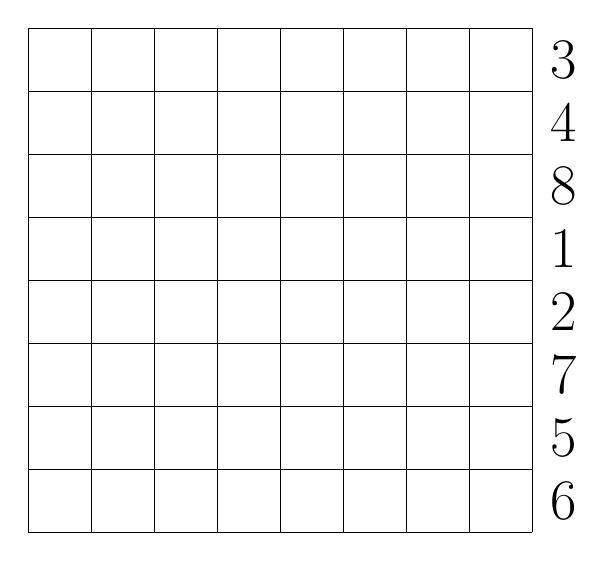
\begin{tikzpicture}[scale = 0.8]
    \foreach \i/\j in {1/3,2/4,3/8,4/1,5/2,6/7,7/5,8/6} {
      \node at (\j - 0.5, 8.5 - \i) {\huge\rook};
      \node at (8.5, 8.5-\i) {\huge\j};
    }
    \draw (0,0) grid (8,8);
  \end{tikzpicture}
  \caption[A permutation corresponding to a rook placement.]{
    An illustration of the rook placement corresponding to the permutation
    $34812756 \in S_8$. A rook is placed in square $(i, \pi(i))$ for each $i$.
  }
  \label{fig:permutationFromRooks}
\end{figure}


\subsection{Definitions in rook theory}
We begin by introducing some preliminary ideas from rook theory.

\begin{definition}
  A \textit{board} $B$ is a subset of $[n] \times [n]$ which represents the
  squares of a $n \times n$ chessboard that rooks are allowed to be placed on.
  Every board $B$ has a \textit{complementary board}
  $B^c = ([n] \times [n]) \setminus B$, which consists of all of the
  squares of $B$ that a rook cannot be placed on.
\end{definition}

To each board, we can associate a generating polynomial that keeps track of the
number of ways to place a given number of rooks on the valid squares in such a
way that no two rooks are in the same row or column.

\begin{definition}
  The \textit{rook polynomial} associated with a board $B$,
  \[
    p_B(x) = r_0 + r_1 x + r_2 x^2 + \dots + r_n x^n,
  \]
  is a generating polynomial where $r_k$ denotes the number of $k$-element subsets
  of $B$ such that no two elements share an $x$-coordinate or a $y$-coordinate.
\end{definition}

In the context of permutations, we're typically interested in $r_n$, the number
of ways to place $n$ rooks on a restricted $n \times n$ board.
However, it turns out that a naive application of the techniques from
rook theory do not immediately allow us to count the number of
restricted permutations with a given prefix.
Computing the number of such permutations is known to be computationally hard
for a board with arbitrary restrictions.
We can see this by encoding a board $B$ as a $(0,1)$-matrix and computing the matrix
permanent. (In fact, Shevelev \cite{Shevelev1992} claims that
``the theory of enumerating the permutations with restricted positions
stimulated the development of the theory of the permanent.'')

\begin{lemma}
  Let $M_B = \{a_{ij}\}$ be an $n \times n$ matrix where \[
    a_{ij} = \begin{cases}
      1 & (i,j) \in B \\
      0 & (i,j) \not\in B
    \end{cases}.
  \]
  Then the coefficient of $x^n$ in $p_B(x)$ is given by the matrix permanent
  \[
    \operatorname{perm}(M_B) = \sum_{\sigma \in S_n} \prod_{i=1}^n a_{i\sigma(i)}.
  \]
\end{lemma}

Now is an appropriate time to recall Valiant's Theorem.

\begin{theorem}[Valiant's Theorem \cite{Valiant1979}]
  Computing the permanent of a (0,1)-matrix is \#P-complete.
\end{theorem}

\begin{corollary}
  Computing the number of rook placements on an arbitrary $n \times n$ board is
  \#P-hard.
\end{corollary}

Therefore, in order to compute the number of permutations, we must exploit some
additional structure of the restrictions.

\subsection{Techniques of Rook Theory}
Rook polynomials can be computed recursively. The base case is that
for an empty board $B = \emptyset$, the corresponding rook polynomial is
$p_\emptyset(x) = 1$, because there is one way to place no rooks, and no way
to place one or more rooks.
\begin{lemma}[\cite{Riordan1980}]
  Given a board, $B$, then for any square $(x,y) \in B$, we can define
  the resulting boards if we include or exclude the square respectively
  \begin{align}
    B_i &= \{(x',y') \in B : x \neq x' \text{ and } y \neq y'\} \\
    B_e &= B \setminus {(x,y)}.
  \end{align}
  Then we can write the rook polynomial for $B$ in terms of this decomposition.
  \[
    p_B(x) = xp_{B_i}(x) + p_{B_e}(x).
  \]
  \label{lemma:rookPolynomialRecursion}
\end{lemma}

If we want to compute a rook polynomial using this construction, we can end
up adding up lots of smaller rook polynomials---a number that is exponential in
the size of $B$.
However, when the number of squares in $B^c$ is small in some sense, it can be
easier to compute the rook polynomial $p_{B^c}$ and use the principle of
inclusion/exclusion on it's coefficients to determine the rook polynomial for
the original board, $B$.

In the case of derangements and m\'enage permutations, this is the strategy
we'll use.
Start by finding the resulting board from a given prefix,
find the rook polynomial of the complementary board, and
use the principle of inclusion/exclusion to determine the number of ways to
place rooks in the resulting board.

\section{Unranking Derangements}

In January 2020, Richard Arratia sent out an email proposing a seminar talk.
The title describes the first ``\$100 problem'':
\begin{problem}
``For $100$ dollars, what is the $500$ quadrillion-th derangement on $n=20$?''
\end{problem}

\begin{answer}
The computer program in Appendix TODO computed the answer in less than ten
milliseconds. When written as words in lexicographic order, the
derangement in $S_{20}$ with rank $5 \times 10^{17}$ is \[
  12\ 14\ 2\ 9\ 13\ 20\ 6\ 3\ 1\ 17\ 5\ 11\ 19\ 15\ 10\ 18\ 8\ 7\ 4\ 16.
\]
\end{answer}

Arratia's question focused on unranking derangements where the rank was
based on the total ordering that comes from writing the
permutations as words in lexicographic order.
Other authors have looked at unranking derangements based on other total
orderings. In particular, Mikawa and Tanaka \cite{Mikawa2014} give an algorithm
to rank/unrank derangements
with respect to \textit{lexicographic ordering in cycle notation}.

In this section we will develop an algorithm for ranking and unranking with
respect to their lexicographic ordering as words. The technique that we use will
broadly be re-used in the next section.
It is worthwhile to begin by recalling the definition of a derangement.
\begin{definition}
  A \textit{derangement} is a permutation $\pi \in S_n$ such that $\pi$ has no
  fixed points. That is, the set of derangements is \[
    \{\pi \in S_n : \pi(i) \neq i\ \forall i \in [n]\}.
  \]
\end{definition}

\subsection{The complementary board.}
In order to compute the number of derangements with a given prefix, it is
useful to look at the board that results after placing $k$ rooks according to
these positions, as illustrated in Figure \ref{fig:derangementPrefix}.

\begin{figure}
  \center
  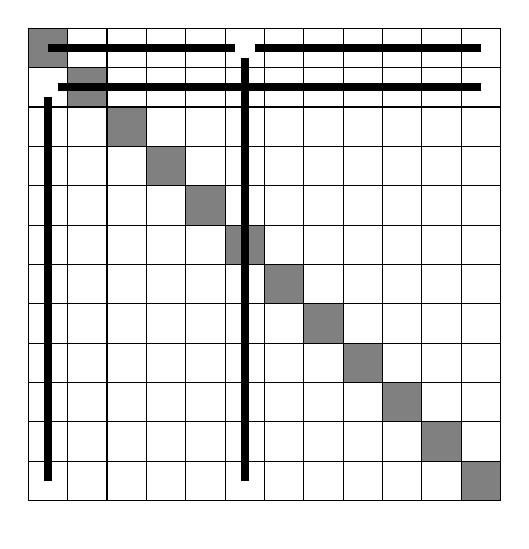
\begin{tikzpicture}[scale = 0.5]
    \path (0,-0.5) -- (0,6.5);
    \foreach \i in {0,...,11} { \fill[gray] (\i, 12-\i) rectangle (\i + 1, 11 - \i); }
    \draw (0,0) grid (12,12);
    \node (R1) at (5.5, 11.5) {\Large\symrook};
    \node (R2) at (0.5, 10.5) {\Large\symrook};
    \draw[line width = 3]
      (0.5,11.5) -- (R1) -- (11.5,11.5)
      (R1) -- (5.5,0.5)
    ;
    \draw[line width = 3]
      (R2) -- (11.5,10.5)
      (R2) -- (0.5,0.5)
    ;
  \end{tikzpicture}
  ~~
  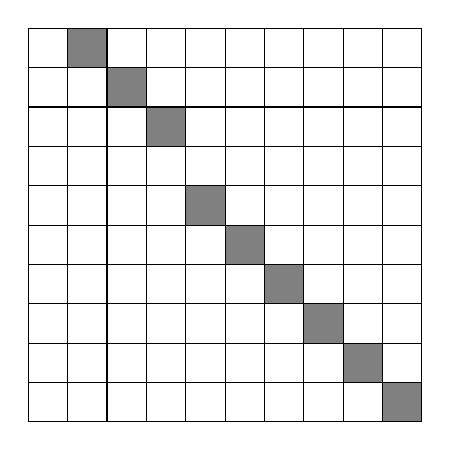
\begin{tikzpicture}[scale = 0.5]
    \path (0,-0.5) -- (0,6.5);
    \foreach \i in {1,...,3} { \fill[gray] (\i, 11-\i) rectangle (\i + 1, 10 - \i); }
    \foreach \i in {4,...,9} { \fill[gray] (\i, 10-\i) rectangle (\i + 1, 9 - \i); }
    \draw (0,0) grid (10,10);
  \end{tikzpicture}
  \caption[The derived board for a prefix of a derangement.]{An example of a prefix $\alpha = (6, 1)$, and the board that results
  from deleting the first $\ell = 2$ rows and columns $6$ and $1$.
  The derived complementary board of $B$ from $\alpha$ is
  $B^c_\alpha = \{(1,2), (2,3), (3,4), (5,5), \dots, (10,10)\}$.}
\label{fig:derangementPrefix}
\end{figure}


\begin{definition}
  If $B$ is an $n \times n$ board, and
  $\alpha = (\alpha_1, \alpha_2, \dots, \alpha_\ell)$ is a valid prefix of length
  $\ell$, then \textbf{derived complementary board} of $B$ from $\alpha$,
  denoted $B^c_\alpha$,
  is $B$ with the appropriate rows and columns removed and reindexed in such
  a way that $B^c_\alpha \subseteq [n - \ell] \times [n - \ell]$.
  % \[
  %   B^c_\alpha \cup \{(x, y) : x \in [n], y \in [\ell]\} \cup \{(x, y) : x \in \alpha, y \in [n]\}
  % \]
  % the \textit{derived complementary board} of $B$ from $\alpha$, denoted
  % $B^c_\alpha \subset [n-k]^2$ consisting of a subset of $B^c$, relabeled to
  % reflect ... TODO
\end{definition}
\begin{lemma}
  Given a valid $\ell$ letter prefix $(\alpha_1, \alpha_2, \dots, \alpha_\ell)$
  of a word on $n$ letters,
  the number of squares in the resulting complementary board is \[
    |B_\alpha^c| = n - \ell - |\{\ell+1, \ell+2, \dots, n\} \cap \{\alpha_1, \alpha_2, \dots, \alpha_\ell\}|,
  \] and no two of these squares are in the same row or column.
\end{lemma}
\begin{proof}
  TODO
  % Recall that $B^c = \{(1,1), (2,2), \dots, (n,n)\}$, so no square shares its
  % first or second coordinate with another square.
  % Because $B^c_\alpha$ is the result of deleting and relabeling the squares of
  % $B^c$, $B^c_\alpha$ also has two squares with with same first or second
  % coordinate.
  % In order to
  % Because the prefix is of length $\ell$, all of the squares in $B_\alpha^c$ must
  % have a first coordinate greater than $\ell$, that is,
  % $B_\alpha^c \subseteq \{(\ell+1, \ell+1), (\ell+2, \ell+2), \dots, (n, n)\}$.
  % Then, we can count how many of these remaining squares are in the same row or
  % column as a rook in the prefix. This number is the size of the intersection
  % $|\{\ell+1, \ell+2, \dots, N\} \cap \{\alpha_1, \alpha_2, \dots, \alpha_p\}|$.
\end{proof}

\subsection{Derangements with a given prefix}
Now that we have a way of quickly computing $|B_\alpha^c|$, we can compute the
number of ways to place $j$ rooks on the complementary board. We can use this
to compute the number of derangements that begin with the prefix $\alpha$.

\begin{lemma}
  The rook polynomial for the complementary board $B_\alpha^c$ is \begin{equation}
    p_{B_\alpha^c}(x) = \sum_{j = 0}^{|B_\alpha^c|} \binom{|B_\alpha^c|}{j}x^j.
  \end{equation}
\end{lemma}
\begin{proof}
  No two squares in $B^c$ (and thus $B^c_\alpha$) are in the same row or column.
  Thus the number of ways to place $j$ rooks is equivalent to selecting $j$
  cells from $|B^c_\alpha|$.
\end{proof}

Now we introduce a lemma of Stanley \cite{Stanley2011EC1} to compute the number
of TODO from a complementary board.

\begin{lemma}[\cite{Stanley2011EC1}]
  The number of ways, $N_0$, of placing $n$ nonattacking rooks on a board
  $B \subseteq [n] \times [n]$ is given by \[
    N_0 = \sum_{k=0}^n (-1)^k r_k (n-k)!,
  \] where $P_{B^c}(x) = \sum_{k=0}^n r_k x^k$.
  \label{lemma:CountsFromComplementaryPolynomials}
\end{lemma}

\begin{corollary}
  The number of derangements with prefix
  $\alpha = (\alpha_1, \alpha_2, \dots, \alpha_\ell)$
  is given by \[
    \#\operatorname{prefix}(\alpha)
    = \sum_{j=0}^{|B_\alpha^c|} (-1)^j \binom{|B_\alpha^c|}{j}(n-\ell-j)!,
  \] which is $\operatorname{A047920}(n-\ell, |B_\alpha^c|)$ in
  the On-Line Encyclopedia of Integer Sequences \cite{oeis}.
\end{corollary}

\begin{example}
  For example, for $N = 14$, we wish to count the number of derangements that
  start with the prefix $6\,1$. Since the prefix has two letters, $p = 2$ and
  $n = 14 - 2 = 12$. The only crossed-out cell that is deleted by the prefix in the
  remaining board is the cell that was in position $6$:
  in particular, $\{3,4,\dots,14\} \cap \{6, 1\} = 6$.
  Thus $k = 12 - 1 = 11$.
  Thus there are $A047920(12,11) = 190\,899\,411$ derangements that start
  with $6\,1$.
\end{example}
\begin{table}
\begin{tabular}{|l|r|l|c|l|}
  \hline
  $\alpha$ (prefix)   & $\operatorname{\#prefix}(\alpha)$ & index range & $|B_\alpha^c|$ & $f^{\mathcal{D}}_i(\alpha, \ell)$ \\
  \hline
  $1       $ & $0$    & $(0,0]$           & $-$ & $f^{\mathcal{D}}_{1000}(1, 0)$          \\
  $2       $ & $2119$ & $(0,2119]$        & $6$ & $f^{\mathcal{D}}_{1000}(2, 0)$          \\
  \hline
  $21      $ & $265$  & $(0, 265]$        & $6$ & $f^{\mathcal{D}}_{1000}(21, 0)$         \\
  $22      $ & $0$    & $(265, 265]$      & $-$ & $f^{\mathcal{D}}_{1000}(22, 265)$       \\
  $23      $ & $309$  & $(265, 574]$      & $5$ & $f^{\mathcal{D}}_{1000}(23, 265)$       \\
  $24      $ & $309$  & $(574, 883]$      & $5$ & $f^{\mathcal{D}}_{1000}(24, 574)$       \\
  $25      $ & $309$  & $(883, 1192]$     & $5$ & $f^{\mathcal{D}}_{1000}(25, 883)$       \\
  \hline
  $251     $ & $53$   & $(883, 936]$      & $4$ & $f^{\mathcal{D}}_{1000}(251, 883)$      \\
  $253     $ & $0$    & $(936, 936]$      & $-$ & $f^{\mathcal{D}}_{1000}(253, 936)$      \\
  $254     $ & $64$   & $(936, 1000]$     & $3$ & $f^{\mathcal{D}}_{1000}(254, 936)$      \\
  \hline
  $2541    $ & $11$   & $(936, 947]$      & $3$ & $f^{\mathcal{D}}_{1000}(2541, 936)$     \\
  $2543    $ & $11$   & $(947, 958]$      & $3$ & $f^{\mathcal{D}}_{1000}(2543, 947)$     \\
  $2546    $ & $14$   & $(958, 972]$      & $2$ & $f^{\mathcal{D}}_{1000}(2546, 958)$     \\
  $2547    $ & $14$   & $(972, 986]$      & $2$ & $f^{\mathcal{D}}_{1000}(2547, 972)$     \\
  $2548    $ & $14$   & $(986, 1000]$     & $2$ & $f^{\mathcal{D}}_{1000}(2548, 986)$     \\
  \hline
  $25481   $ & $3$    & $(986, 989]$      & $2$ & $f^{\mathcal{D}}_{1000}(25481, 986)$    \\
  $25483   $ & $3$    & $(989, 992]$      & $2$ & $f^{\mathcal{D}}_{1000}(25483, 989)$    \\
  $25486   $ & $4$    & $(992, 996]$      & $1$ & $f^{\mathcal{D}}_{1000}(25486, 992)$    \\
  $25487   $ & $4$    & $(996, 1000]$     & $1$ & $f^{\mathcal{D}}_{1000}(25487, 996)$    \\
  \hline
  $254871   $ & $2$   & $(996, 998]$      & $0$ & $f^{\mathcal{D}}_{1000}(254871, 996)$   \\
  $254873   $ & $2$   & $(998, 1000]$     & $0$ & $f^{\mathcal{D}}_{1000}(254873, 998)$   \\
  \hline
  $2548731  $ & $1$   & $(998, 999]$      & $0$ & $f^{\mathcal{D}}_{1000}(2548731, 998)$  \\
  $2548736  $ & $1$   & $(999, 1000]$     & $0$ & $f^{\mathcal{D}}_{1000}(2548736, 999)$  \\
  \hline
  $25487361 $ & $1$   & $(999, 1000]$     & $0$ & $f^{\mathcal{D}}_{1000}(25487361, 999)$ \\
  \hline
\end{tabular}
\caption[Steps for computing the $1000$th derangement in $S_8$]{
  There are $A000166(8) = 14833$ derangements on $8$ letters.
  This algorithm finds the derangement at index $1000$.
}
\end{table}

% %%%%%%%%%%%%%%%%%%%%%%%%%%%%%%%%%%%%%%%%%%%%%
% Section 3
% %%%%%%%%%%%%%%%%%%%%%%%%%%%%%%%%%%%%%%%%%%%%%
\section{Unranking M\'enage Permutations}

\subsection{Proof of concept (The \$100 answer!)}
In February 2020, Richard Arratia offered
\begin{problem}
  For $n=20$ there are $A000179(20) = 312\,400\,218\,671\,253\,762 > 3.1\cdot 10^{17}$
  m\'enage permutations.
  Determine the $10^{17}$-th such permutation when listed in lexicographic order.
\end{problem}
\begin{answer}
  The desired permutation is \begin{equation}
    7\ 16\ 19\ 12\ 2\ 8\ 15\ 1\ 18\ 14\ 3\ 9\ 20\ 10\ 5\ 17\ 13\ 4\ 11\ 6.
  \end{equation}
\end{answer}

A M\'enage permutation comes from the \textit{problème des ménages}. % https://en.wikipedia.org/wiki/M%C3%A9nage_problem
Here we will define it as
\begin{definition}
  A \textit{m\'enage permutation} is a permutation $\pi \in S_n$ such that for
  all $i \in [n]$,
  $\pi(i) \neq i$ and
  $\pi(i) + 1 \not\equiv i \bmod n$.
\end{definition}

We can use the prefix to get a new board, which is block diagonal
(whenever the prefix is non-empty), if we know the number of cells in each
block, we can compute the number of valid boards. This gives us the number of
m\'enage permutations with a given prefix.

Prefix $\Rightarrow$ grouped columns $\Rightarrow$ partition/multiset $\Rightarrow$ complementary polynomial $\Rightarrow$ count

\subsection{Block diagonal decomposition}
When we look at Figure TODO, it appears that placing rooks according to a prefix
results in a derived complementary board where the squares can be grouped into
sub-boards that don't share any rows or columns. We will see that this property
holds more generally, and we can exploit this in order to describe the number
of m\'enage permutations with a given prefix.

It is useful to begin by formalizing this notion of grouping squares.
\begin{definition}
  Two boards $B$ and $B'$ are called \textbf{disjoint} if no squares of $B$ are
  in the same row or column as any square in $B'$.
\end{definition}

The reason that we care about decomposing a board into disjoint parts
is because that perspective allows us to factor the rook polynomial.
\begin{theorem}[\cite{Kaplansky1946}]
  If $B$ can be partitioned into disjoint boards $b_1, b_2, \dots, b_m$,
  then the rook polynomial of $B$ is the product of the rook polynomials of
  the $b_i$s \[
    p_B(x) = \prod_{i=1}^m p_{b_i}(x).
  \]
\end{theorem}

This disjoint decomposition is useful for this context because,
as Figure \ref{fig:menageSinglePlacement} suggests, the derived
complementary board for a nonempty prefix is block-diagonal,
with well-understood blocks.

\begin{figure}[ht!]
  \center
  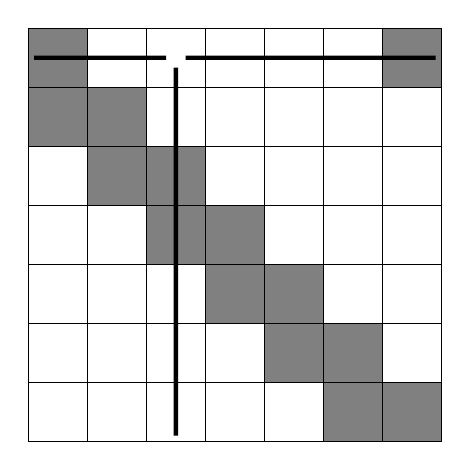
\begin{tikzpicture}[scale = 0.75]
    \foreach \i in {0,...,6} { \fill[gray] (\i, 6 - \i) rectangle (\i + 1, 7 - \i); }
    \foreach \i in {1,...,6} { \fill[gray] (\i-1, 6 - \i) rectangle (\i, 7 - \i); }
    \fill[gray] (6, 6) rectangle (7, 7);
    \draw (0,0) grid (7,7);
    \node (R) at (2.5, 6.5) {\huge\symrook};
    \draw[ultra thick]
      (0.1,6.5) -- (R) -- (6.9,6.5)
      (R) -- (2.5,0.1)
    ;
  \end{tikzpicture}
  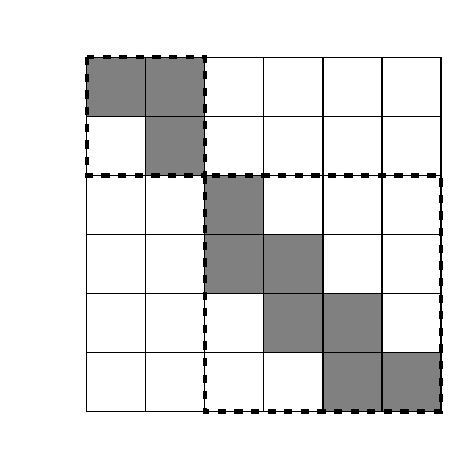
\begin{tikzpicture}[scale = 0.75]
    \path (0,-0.5) -- (0,6.5); % vertically center.
    \foreach \i/\j in {1/5, 2/5, 2/4, 3/3, 3/2, 4/2, 4/1, 5/1, 5/0, 6/0} { \fill[gray] (\i, \j) rectangle (\i + 1, \j + 1); }
    \draw[ultra thick, dashed] (1,6) rectangle (3,4) rectangle (7,0);
    \draw (1,0) grid (7,6);
  \end{tikzpicture}
  \caption[The derived board for a prefix of a m\'enage permutation of length $1$.]{
    The first chessboard shows a placement of a rook at position $3$,
    the second shows the remaining squares, and the third shows a permutation
    of the rows to put the board into a block-diagonal form.
  }
  \label{fig:menageSinglePlacement}
\end{figure}


Now we will give a name to these blocks,
which are illustrated in Figure \ref{fig:blockShape}.

\begin{definition}
  A board is called \textbf{staircase-shaped} if it matches one of the
  following four shapes:
  \begin{alignat*}{2}
    \mathcal{O}_{2n-1}           &= \{(i,i) : i \in [n]\}    &&\cup\ \{(i,i+1) : i \in [n-1]\} \\
    \mathcal{O}_{2n-1}^\intercal &= \{(i,i) : i \in [n]\}    &&\cup\ \{(i+1,i) : i \in [n-1]\} \\
    \mathcal{E}_{2n-2}           &= \{(i,i) : i \in [n-1]\}\ &&\cup\ \{(i+1,i) : i \in [n-1]\} \\
    \mathcal{E}_{2n-2}^\intercal &= \{(i,i) : i \in [n-1]\}\ &&\cup\ \{(i,i+1) : i \in [n-1]\},
  \end{alignat*}
  the subscripts represent the number of cells, and the names represent their
  parity.
  \label{def:staircaseShaped}
\end{definition}

\begin{lemma}
  For $\ell \geq 1$, and prefix $\alpha = (\alpha_1, \alpha_2, \dots, \alpha_\ell)$
  the derived complementary board $B_\alpha^c$ can be partitioned into
  disjoint staircase-shaped boards.
  \label{lemma:boardShape}
\end{lemma}
\begin{proof}
  The proof proceeds by induction on the length of the prefix.

  To establish the base case, consider a prefix of length $\ell = 1$.
  Because of the m\'enage restriction,
  $\alpha_1 \in \{2, 3, \dots, n-1\}$, and
  the derived complimentary board $B_{(\alpha_1)}^c$
  can be partitioned into two disjoint blocks with shapes
  $A_{\alpha_1 - 1}$ and $A^\intercal_{n - \alpha_1}$.
  (This is illustrated for the case of $n = 7$ and $\alpha_1$ in Figure \ref{fig:menageSinglePlacement}.)

  The inductive hypothesis is that the derived complimentary board for
  a prefix of length $\ell - 1$ consists of blocks with shape
  $A_{n_1}$, $A^\intercal_{n_2}$, $B_{n_3}$, or $B^\intercal_{n_4}$.
  Placing a rook in row $\ell$ can remove a top row or a column or both in a
  given block.
  Table \ref{table:rooksInBlocks} below
  shows the resulting blocks after placing a rook in
  $\ell$-th row of $B$,
  which may be in the top row or the $i$-th column of a given block.

  \begin{tabular}{|l|l|l|l|l|}
  \hline
  Rook placement
    & $\mathcal{O}_{2n-1}$
    & $\mathcal{O}_{2n-1}^\intercal$
    & $\mathcal{E}_{2n-2}$
    & $\mathcal{E}_{2n-2}$
  \\ \hline
  Row $1$
    & $\mathcal{O}_{2n-3}$
    & $\mathcal{E}_{2n-2}^\intercal$
    & $\mathcal{O}_{2n-3}$
    & $\mathcal{E}_{2n-4}^\intercal$
  \\
  Column $i$
    & $\mathcal{O}_{2i-3}$, $\mathcal{E}_{2n-2i}$
    & $\mathcal{E}_{2i-2}$, $\mathcal{O}_{2n-2i-1}^\intercal$
    & $\mathcal{E}_{2i-2}$, $\mathcal{E}_{2n-2i-2}$
    & $\mathcal{O}_{2i-3}$, $\mathcal{O}_{2n-2i-1}^\intercal$
  \\
  Row $1$, column $i$
    & $\mathcal{O}_{2i-5}$, $\mathcal{E}_{2n-2i}$
    & $\mathcal{O}_{2i-3}$, $\mathcal{O}_{2n-2i-1}^\intercal$
    & $\mathcal{O}_{2i-3}$, $\mathcal{E}_{2n-2i-2}$
    & $\mathcal{O}_{2i-5}$, $\mathcal{O}_{2n-2i-1}^\intercal$
  \\ \hline
  \end{tabular}
  \captionof{table}{
    The results of placing a rook in the first row, $i$-th column, or both
    for all staircase-shaped boards.
  }
  \label{table:rooksInBlocks}
  Therefore placing any number of rooks in the first $\ell$ results in a board
  of one of the four described shapes.
\end{proof}

\begin{figure}[ht!]
  \center
  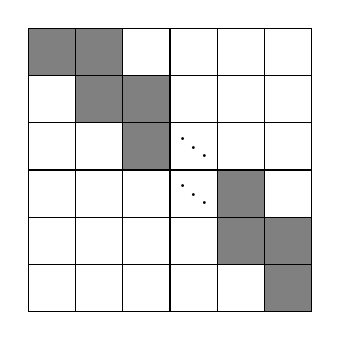
\begin{tikzpicture}[scale=0.6]
    \foreach \i/\j in {1/5, 2/5, 2/4, 3/4, 3/3, 5/2, 5/1, 6/1, 6/0} { \fill[gray] (\i, \j) rectangle (\i + 1, \j + 1); }
    \node at (4.5,3.65) {$\ddots$};
    \node at (4.5,2.65) {$\ddots$};
    \draw (1,0) grid (7,6);
  \end{tikzpicture}
  ~
  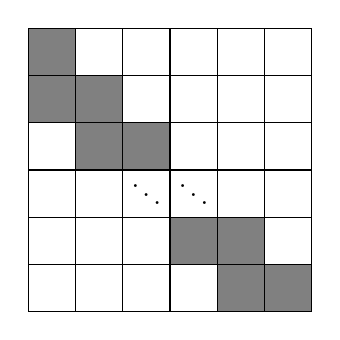
\begin{tikzpicture}[scale=0.6]
    \foreach \i/\j in {1/5, 1/4, 2/4, 2/3, 3/3, 4/1, 5/1, 5/0, 6/0} { \fill[gray] (\i, \j) rectangle (\i + 1, \j + 1); }
    \node at (3.5,2.65) {$\ddots$};
    \node at (4.5,2.65) {$\ddots$};
    \draw (1,0) grid (7,6);
  \end{tikzpicture}
  ~
  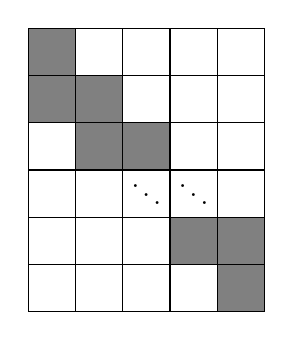
\begin{tikzpicture}[scale=0.6]
    \foreach \i/\j in {1/4, 1/5, 2/3, 2/4, 3/3, 4/1, 5/0, 5/1} { \fill[gray] (\i, \j) rectangle (\i + 1, \j + 1); }
    \node at (3.5,2.65) {$\ddots$};
    \node at (4.5,2.65) {$\ddots$};
    \draw (1,0) grid (6,6);
  \end{tikzpicture}
  ~
  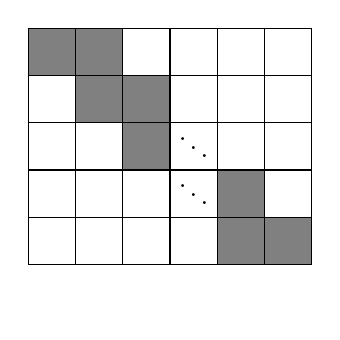
\begin{tikzpicture}[scale=0.6]
    \foreach \i/\j in {1/5, 2/5, 2/4, 3/4, 3/3, 5/2, 5/1, 6/1} { \fill[gray] (\i, \j) rectangle (\i + 1, \j + 1); }
    \node at (4.5,3.65) {$\ddots$};
    \node at (4.5,2.65) {$\ddots$};
    \path (1,0) grid (7,6);
    \draw (1,1) grid (7,6);
  \end{tikzpicture}
  \caption[Block shapes for a m\'enage permutation.]{
    Four boards, two $n \times n$ board with $2n - 1$ grey cells,
    a $n \times n-1$ board with $2n - 2$ grey cells, and a
    $n-1 \times n$ board with $2n - 2$ grey cells.
    We call them $A_n$, $A^\top_n$, $B_n$, and $B^\top_n$ respectively.
  }
  \label{fig:blockShape}
\end{figure}


\subsection{Rook polynomials of blocks}
Recall that the goal of partitioning $B$ into disjoint boards $b_1, b_2, \dots, b_m$
is so that we can factor $p_B(x)$ in terms of $p_{b_i}(x)$. Of course, this is
only helpful if we can describe $p_{b_i}(x)$, which is the goal of this section.
Thankfully, the rook polynomial of each $b_i$ will turn out to depend only on the
number of squares, $|b_i|$, which can be computed easily because of its structure.

We will begin by defining a family of polynomials that, suggestively, will turn
out to be the rook polynomials that we are looking for. This family is nearly
described by OEIS sequence A011973 \cite{oeis}.
\begin{definition}
  For $j \geq 0$, the $j$th \textbf{Fibonacci polynomial} $F_{j}(x)$ is defined recursively as:
  \begin{align}
    F_0(x) &= 1 \\
    F_1(x) &= 1 + x \\
    F_n(x) &= F_{n-1}(x) + xF_{n-2}(x).
  \end{align}
\end{definition}

\begin{lemma}
  If $B$ is a staircase-shaped board with $k$ squares, then
  $B$ has rook polynomial $p_{B}(x) = F_{k}(x)$ which agrees with the $k$-th
  Fibonacci polynomial.
\end{lemma}
\begin{proof}
  We will recall the recursive construction of rook polynomials from
  Lemma \ref{lemma:rookPolynomialRecursion}, and proceed by
  induction on the number of squares, always choosing to include or exclude
  the upper-left square.

  Since the reflections of board has the same rook polynomial as the
  unreflected board, without loss of generality, we
  will compute the rook polynomials for
  $\mathcal{O}_{2n-1}$ and $\mathcal{E}_{2n-2}$ respectively.

  % $A_n$ as our choice for the odd case and
  % $B_n$ as our choice for the even case.

  To establish a base case, consider the rook polynomials when $n = 1$, so
  the even board has $|\mathcal{E}_{0}| = 0$ squares and
  the odd board has $|\mathcal{O}_{1}| = 1$ square.
  We can see the corresponding rook polynomials directly. There is $1$ way to
  place $0$ rooks on $\mathcal{E}_{0}$ and no ways to place more rooks;
  similarly there is
  $1$ way to place $0$ rooks on $\mathcal{O}_{1}$,
  $1$ way to place $1$ rooks on $\mathcal{O}_{1}$, and
  no ways to place more than one rook. Thus \begin{alignat}{2}
    p_{\mathcal{E}_{0}}(x) &= 1     &&= F_0(x), \text{ and} \\
    p_{\mathcal{O}_{1}}(x) &= 1 + x &&= F_1(x).
  \end{alignat}

  With the base case established, our inductive hypothesis is that
  $p_{B}(x) = F_{h}(x)$ for
  whenever $B$ is a
  staircase-shaped boards with $h < k$ squares.



  % Even case
  Assume that we have $k$ squares where $k$ is even, so our board looks like
  $\mathcal{E}_{k}$. We can either place a rook or not in the upper-left square.
  If we include the square, then $(\mathcal{E}_{k})_i \cong \mathcal{E}_{k-2}$,
  if we exclude the square, then $(\mathcal{E}_{k})_e \cong \mathcal{O}_{k-1}$.
  Thus by Lemma \ref{lemma:rookPolynomialRecursion}, the rook polynomial of
  $\mathcal{E}_{k}$ is
  \begin{align}
    p_{\mathcal{E}_{k}}(x)
    &= xp_{\mathcal{E}_{k-2}}(x) + p_{\mathcal{O}_{k-1}}(x) \\
    &= xF_{k-2}(x) + F_{k-1}(x) \\
    &= F_{k}(x).
  \end{align}

  % Odd case
  The case where $k$ is odd proceeds in almost the same way.
  Here our board looks like $\mathcal{O}_{k}$.
  We can either place a rook or not in the upper-left square.
  If we include the square, then $(\mathcal{O}_{k})_i \cong \mathcal{O}_{k-2}$,
  if we exclude the square, then $(\mathcal{O}_{k})_e \cong \mathcal{E}_{k-1}$.
  Again by Lemma \ref{lemma:rookPolynomialRecursion}, the rook polynomial
  of $\mathcal{O}_{k}$ is
  \begin{align}
    p_{\mathcal{O}_{k}}(x)
    &= xp_{\mathcal{O}_{k-2}}(x) + p_{\mathcal{E}_{k-1}}(x) \\
    &= xF_{k-2}(x) + F_{k-1}(x) \\
    &= F_{k}(x).
  \end{align}
\end{proof}

\subsection{Prefix to block sizes}
Here's the idea: we group the uncrossed columns.

\begin{lemma}
  Given a prefix $\alpha = (\alpha_1, \alpha_2, \dots, \alpha_\ell)$
  and $i \not\in \alpha$,
  the number of cells of $B^c$ in column $i$ that do not have
  a first coordinate in $[\ell]$
  is given by the rule:
  \begin{equation}
    c_i = \begin{cases}
      0 & i < \ell \\
      1 & i = k \text{ or } i = n \\
      2 & \ell < i < n
    \end{cases}
  \end{equation}
\end{lemma}

\begin{proof}
  TODO: This almost follows from the description?
\end{proof}

Now we can put these column counts together based on the continuous blocks.

\begin{lemma}
  TODO:
  Partition $[n] \setminus \alpha$ into contiguous parts.
  This naturally partitions $B^c_\alpha$ into disjoint boards.
  The size of these boards is $\sum_{x \in \textrm{part}} c_x$.
  (this is what I've been calling our ``composition'')
\end{lemma}

\begin{figure}[ht!]
  \center
  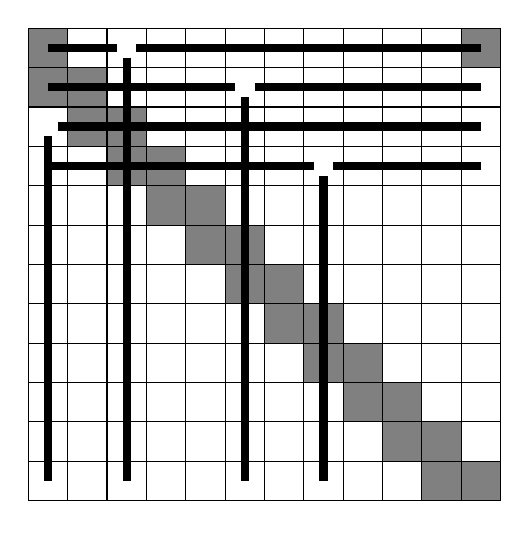
\begin{tikzpicture}[scale = 0.5]
    \path (0,-0.5) -- (0,6.5);
    \foreach \i in {0,...,11} { \fill[gray] (\i, 12-\i) rectangle (\i + 1, 11 - \i); }
    \foreach \i in {0,...,10} { \fill[gray] (\i, 11-\i) rectangle (\i + 1, 10 - \i); }
    \fill[gray] (11,11) rectangle (12,12);
    \draw (0,0) grid (12,12);
    \node (R1) at (2.5, 11.5) {\Large\symrook};
    \node (R2) at (5.5, 10.5) {\Large\symrook};
    \node (R3) at (0.5, 9.5) {\Large\symrook};
    \node (R4) at (7.5, 8.5) {\Large\symrook};
    \draw[line width = 3]
      (0.5,11.5) -- (R1) -- (11.5,11.5)
      (R1) -- (2.5,0.5)
    ;
    \draw[line width = 3]
      (0.5,10.5) -- (R2) -- (11.5,10.5)
      (R2) -- (5.5,0.5)
    ;
    \draw[line width = 3]
      (R3) -- (11.5,9.5)
      (R3) -- (0.5,0.5)
    ;
    \draw[line width = 3]
      (0.5,8.5) -- (R4) -- (11.5,8.5)
      (R4) -- (7.5,0.5)
    ;
  \end{tikzpicture}
  ~~~
  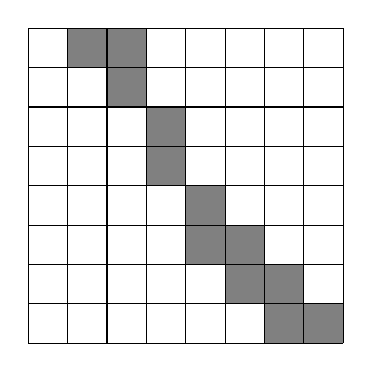
\begin{tikzpicture}[scale = 0.5]
    \path (0,-0.5) -- (0,6.5);
    \foreach \i/\j in {1/7, 2/6, 2/7, 3/4, 3/5, 4/2, 4/3, 5/2, 5/1, 6/1, 6/0, 7/0} {
      \fill[gray] (\i, \j) rectangle (\i + 1, \j + 1);
    }
    \draw (0,0) grid (8,8);
  \end{tikzpicture}
  ~~~
  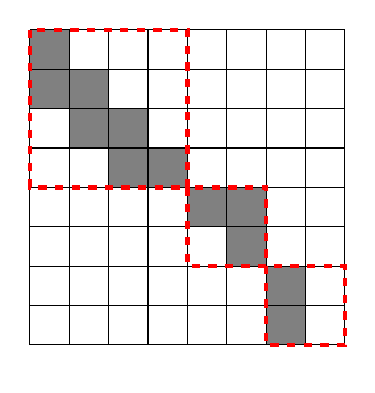
\begin{tikzpicture}[scale = 0.5]
    \path (0,-0.5) -- (0,6.5);
    \foreach \i/\j in {0/7, 0/6, 1/6, 1/5, 2/5, 2/4, 3/4, 4/3, 5/3, 5/2, 6/1, 6/0} {
      \fill[gray] (\i, \j) rectangle (\i + 1, \j + 1);
    }
    \draw (0,0) grid (8,8);
    \draw[ultra thick, dashed, red]
      (0,8) rectangle (4,4)
      (4,4) rectangle (6,2)
      (6,2) rectangle (8,0)
    ;
  \end{tikzpicture}
  \caption{
    xxx
  }
  \label{fig:partitionFromPrefix}
\end{figure}


\subsection{Complementary polynomials to m\'enage permutations with a given prefix}
Recap: We've taken a prefix, used it to find contiguous regions, used these to
find disjoint sub-boards related to $B_\alpha^c$, whose rook polynomials we know.
Now it's time to take these to count our number of m\'enage permutations with
the aforementioned prefix.
\begin{lemma}
  Given a board $B_\alpha^c$ that is partitioned into disjoint boards
  $b_1, b_2, \dots, b_m$, the rook polynomial of $B_\alpha^c$ is \[
    p_{B_\alpha^c}(x) = \prod_{i = 1}^m F_{b_i}(x).
  \]
\end{lemma}
\begin{proof}
  This follows directly from Lemma (TODO: rook polynomials of blocks)
  and Lemma (TODO: product of blocks is whole thing).
\end{proof}

Now that we know $p_{B_\alpha^c}$, we can use Lemma
(TODO: Complementary to original) to determine how many
m\'enage permutations there are with a given prefix. Because of Lemma
(TODO: all we need is the prefix to unrank), we have an algorithm to unrank.

\begin{example}
  Illustrating this particular example is too big to be of much interest, so
  here's a smaller example. There are $A000179(8) = 4738$ m\'enage
  permutations on $8$ letters. We'll use this algorithm to find the one
  at index $1000$.
  \begin{table}
    \center
    \begin{tabular}{|l|r|l|c|l|}
      \hline
      $\alpha$ & $\#\operatorname{prefix}(\alpha)$ & index range & composition & $\operatorname{unrank}_{i}(\alpha, \ell)$\\ \hline
      $1       $ & $0$   & $(0,0]$            & $-$       & $\operatorname{unrank}_{1000}(1,0)$          \\
      $2       $ & $787$ & $(0,787]$          & $(1,11)$  & $\operatorname{unrank}_{1000}(2,0)$          \\
      $3       $ & $791$ & $(787, 1578]$      & $(3,9)$   & $\operatorname{unrank}_{1000}(3,787)$        \\ \hline
      $31      $ & $0$   & $(787, 787]$       & $-$       & $\operatorname{unrank}_{1000}(31,787)$       \\
      $32      $ & $0$   & $(787, 787]$       & $-$       & $\operatorname{unrank}_{1000}(32,787)$       \\
      $33      $ & $0$   & $(787, 787]$       & $-$       & $\operatorname{unrank}_{1000}(33,787)$       \\
      $34      $ & $159$ & $(787, 946]$       & $(1,7)$   & $\operatorname{unrank}_{1000}(34,787)$       \\
      $35      $ & $166$ & $(946, 1112]$      & $(1,2,5)$ & $\operatorname{unrank}_{1000}(35,946)$       \\ \hline
      $351     $ & $24$  & $(946, 970]$       & $(0,2,5)$ & $\operatorname{unrank}_{1000}(351,946)$      \\
      $\cdots$   & $0$   & $(970,970]$        & $-$       & \\
      $354     $ & $34$  & $(970, 1004]$      & $(0,5)$   & $\operatorname{unrank}_{1000}(354,970)$      \\ \hline
      $3541    $ & $5$   & $(970,975]$        & $(0,5)$   & $\operatorname{unrank}_{1000}(3541,970)$     \\
      $3542    $ & $5$   & $(975,980]$        & $(0,5)$   & $\operatorname{unrank}_{1000}(3542,975)$     \\
      $\cdots$   & $0$   & $(980,980]$        & $-$       & \\
      $3546    $ & $8$   & $(980,988]$        & $(0,3)$   & $\operatorname{unrank}_{1000}(3546,980)$     \\
      $3547    $ & $10$  & $(988,998]$        & $(0,2,1)$ & $\operatorname{unrank}_{1000}(3547,988)$     \\
      $3548    $ & $6$   & $(998,1004]$       & $(0,4)$   & $\operatorname{unrank}_{1000}(3548,998)$     \\ \hline
      $35481   $ & $1$   & $(998,999]$        & $(0,4)$   & $\operatorname{unrank}_{1000}(35481,998)$    \\
      $35482   $ & $1$   & $(999,1000]$       & $(0,4)$   & $\operatorname{unrank}_{1000}(35482,999)$    \\ \hline
      $354821  $ & $0$   & $(999,999]$        & $(3)$     & $\operatorname{unrank}_{1000}(354821,999)$   \\
      $\cdots$   & $0$   & $(999,999]$        & $-$       & \\
      $354827  $ & $1$   & $(999,1000]$       & $(0,1)$   & $\operatorname{unrank}_{1000}(354827,999)$   \\ \hline
      $3548271 $ & $1$   & $(999,1000]$       & $(0)$     & $\operatorname{unrank}_{1000}(3548271,999)$  \\ \hline
      $35482716$ & $1$   & $(999,1000]$       & $()$      & $\operatorname{unrank}_{1000}(35482716,999)$ \\ \hline
    \end{tabular}
    \caption[Steps for computing the $1000$th m\'enage permutation in $S_8$.]{
      The recursive computation of the 1000th m\'enage permutation.
    }
  \end{table}
\end{example}

\section{Generalizations and Open Questions}
\subsection{Other restricted permutations}
Doron Zeilberger considers a more general family of restricted permutations.
\begin{definition}[\cite{Zeilberger2014}]
  Let $S \subset \mathbb Z$, then a \textit{$S$-avoiding permutation} is a
  permutation $\pi \in S_n$ such that \[
    \pi(i) - i - s \not\equiv 0 \bmod n \text{ for all } i \in [n] \text{ and } s \in S.
  \]
\end{definition}

\begin{example}
  Ordinary permutations are $\emptyset$-avoiding permutations,
  derangements are $\{0\}$-avoiding permutations, and
  we've defined menag\'e permutations as $\{-1,0\}$-avoiding permutations.

  The results in this paper generalize pretty easily to $\{i,i+1\}$-avoiding
  permutations for all $i$.
\end{example}

\subsection{Observation about Lyndon Words after? a given prefix}
\begin{definition}
  A \textit{Lyndon word} is a string that is the unique minimum with respect
  to all of its rotations.
\end{definition}
\begin{example}
  $00101$ is a Lyndon word because
  $00101 = \min\{00101, 01010, 10100, 01001, 10010\}$ is the unique minimum of
  all of its rotations.

  $011011$ is not a Lyndon word because while $011011 = \min\{011011, 110110, 101101, 011011, 110110, 101101\}$,
  it is not the \textbf{unique} minimum.
\end{example}
\begin{conjecture}
  Let $\mathcal{E}^{-1}$ denote the inverse Euler transform.
  Then the number of length $n+1$ Lyndon words that start with a prefix
  $\alpha$ follows a ``simple'' linear recurrence for sufficiently large $n$.
\end{conjecture}
